\documentclass[tikz, border=3mm]{standalone}
\usepackage{tikz}
\usetikzlibrary{arrows.meta, decorations.markings, angles, quotes, calc}

\begin{document}
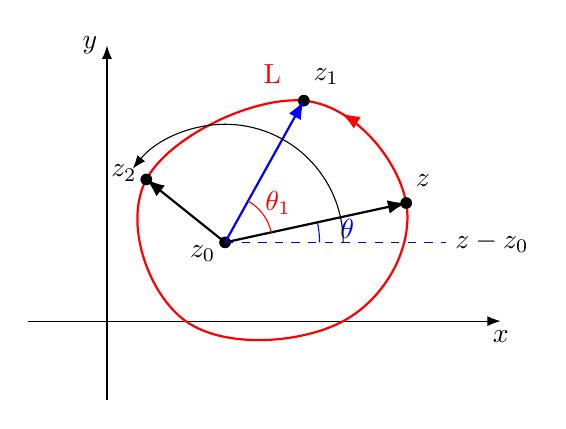
\begin{tikzpicture}[
    >=Latex, % Set default arrow tip style
    dot/.style={fill=black, circle, inner sep=1.5pt} % Style for points
]

% Axes
\draw[->] (-1, 0) -- (5, 0) node[below] {$x$};
\draw[->] (0, -1) -- (0, 3.5) node[left] {$y$};

% Define coordinates
\coordinate (z0) at (1.5, 1);
\coordinate (z)  at (3.8, 1.5);
\coordinate (z1) at (2.5, 2.8);
\coordinate (z2) at (0.5, 1.8);

% Draw the closed curve L
\draw[red, thick,
    postaction={decorate, decoration={markings, mark=at position 0.95 with {\arrow{>}}}} % Counter-clockwise arrow
] plot [smooth cycle, tension=0.7] coordinates {(z) (z1) (z2) (1,0) (3,0)};
\node[red, above] at (2.1, 2.9) {L}; % Label L

% Draw points
\node[dot, label={[below left]$z_0$}] at (z0) {};
\node[dot, label={[above right]$z$}] at (z) {};
\node[dot, label={[above right]$z_1$}] at (z1) {};
\node[dot, label={[ left]$z_2$}] at (z2) {};

% Draw vectors from z0
\draw[->, thick, blue] (z0) -- (z1);
\draw[->, thick] (z0) -- (z);
\draw[->, thick] (z0) -- (z2);

% Draw dashed horizontal line and label
\coordinate (z0_horz_end) at ($(z0)+(2.8,0)$); % Point to the right of z0 for angle/line
\draw[dashed, blue] (z0) -- (z0_horz_end) node[right, black] {$z-z_0$};

% Draw angles using angles library
% Angle theta
\pic [draw, angle radius=1.2cm, "$\theta$", blue, angle eccentricity=1.3] {angle = z0_horz_end--z0--z};
% Angle theta_1
\pic [draw, angle radius=0.6cm, "$\theta_1$", red, angle eccentricity=1.4] {angle = z--z0--z1};
% Angle for z2 (larger arc)
\pic [draw, ->, angle radius=1.5cm] {angle = z0_horz_end--z0--z2};

\end{tikzpicture}
\end{document}